\begin{figure*}[ht!]
    \centering
    \vspace{-2.6cm}
    \centerline{
        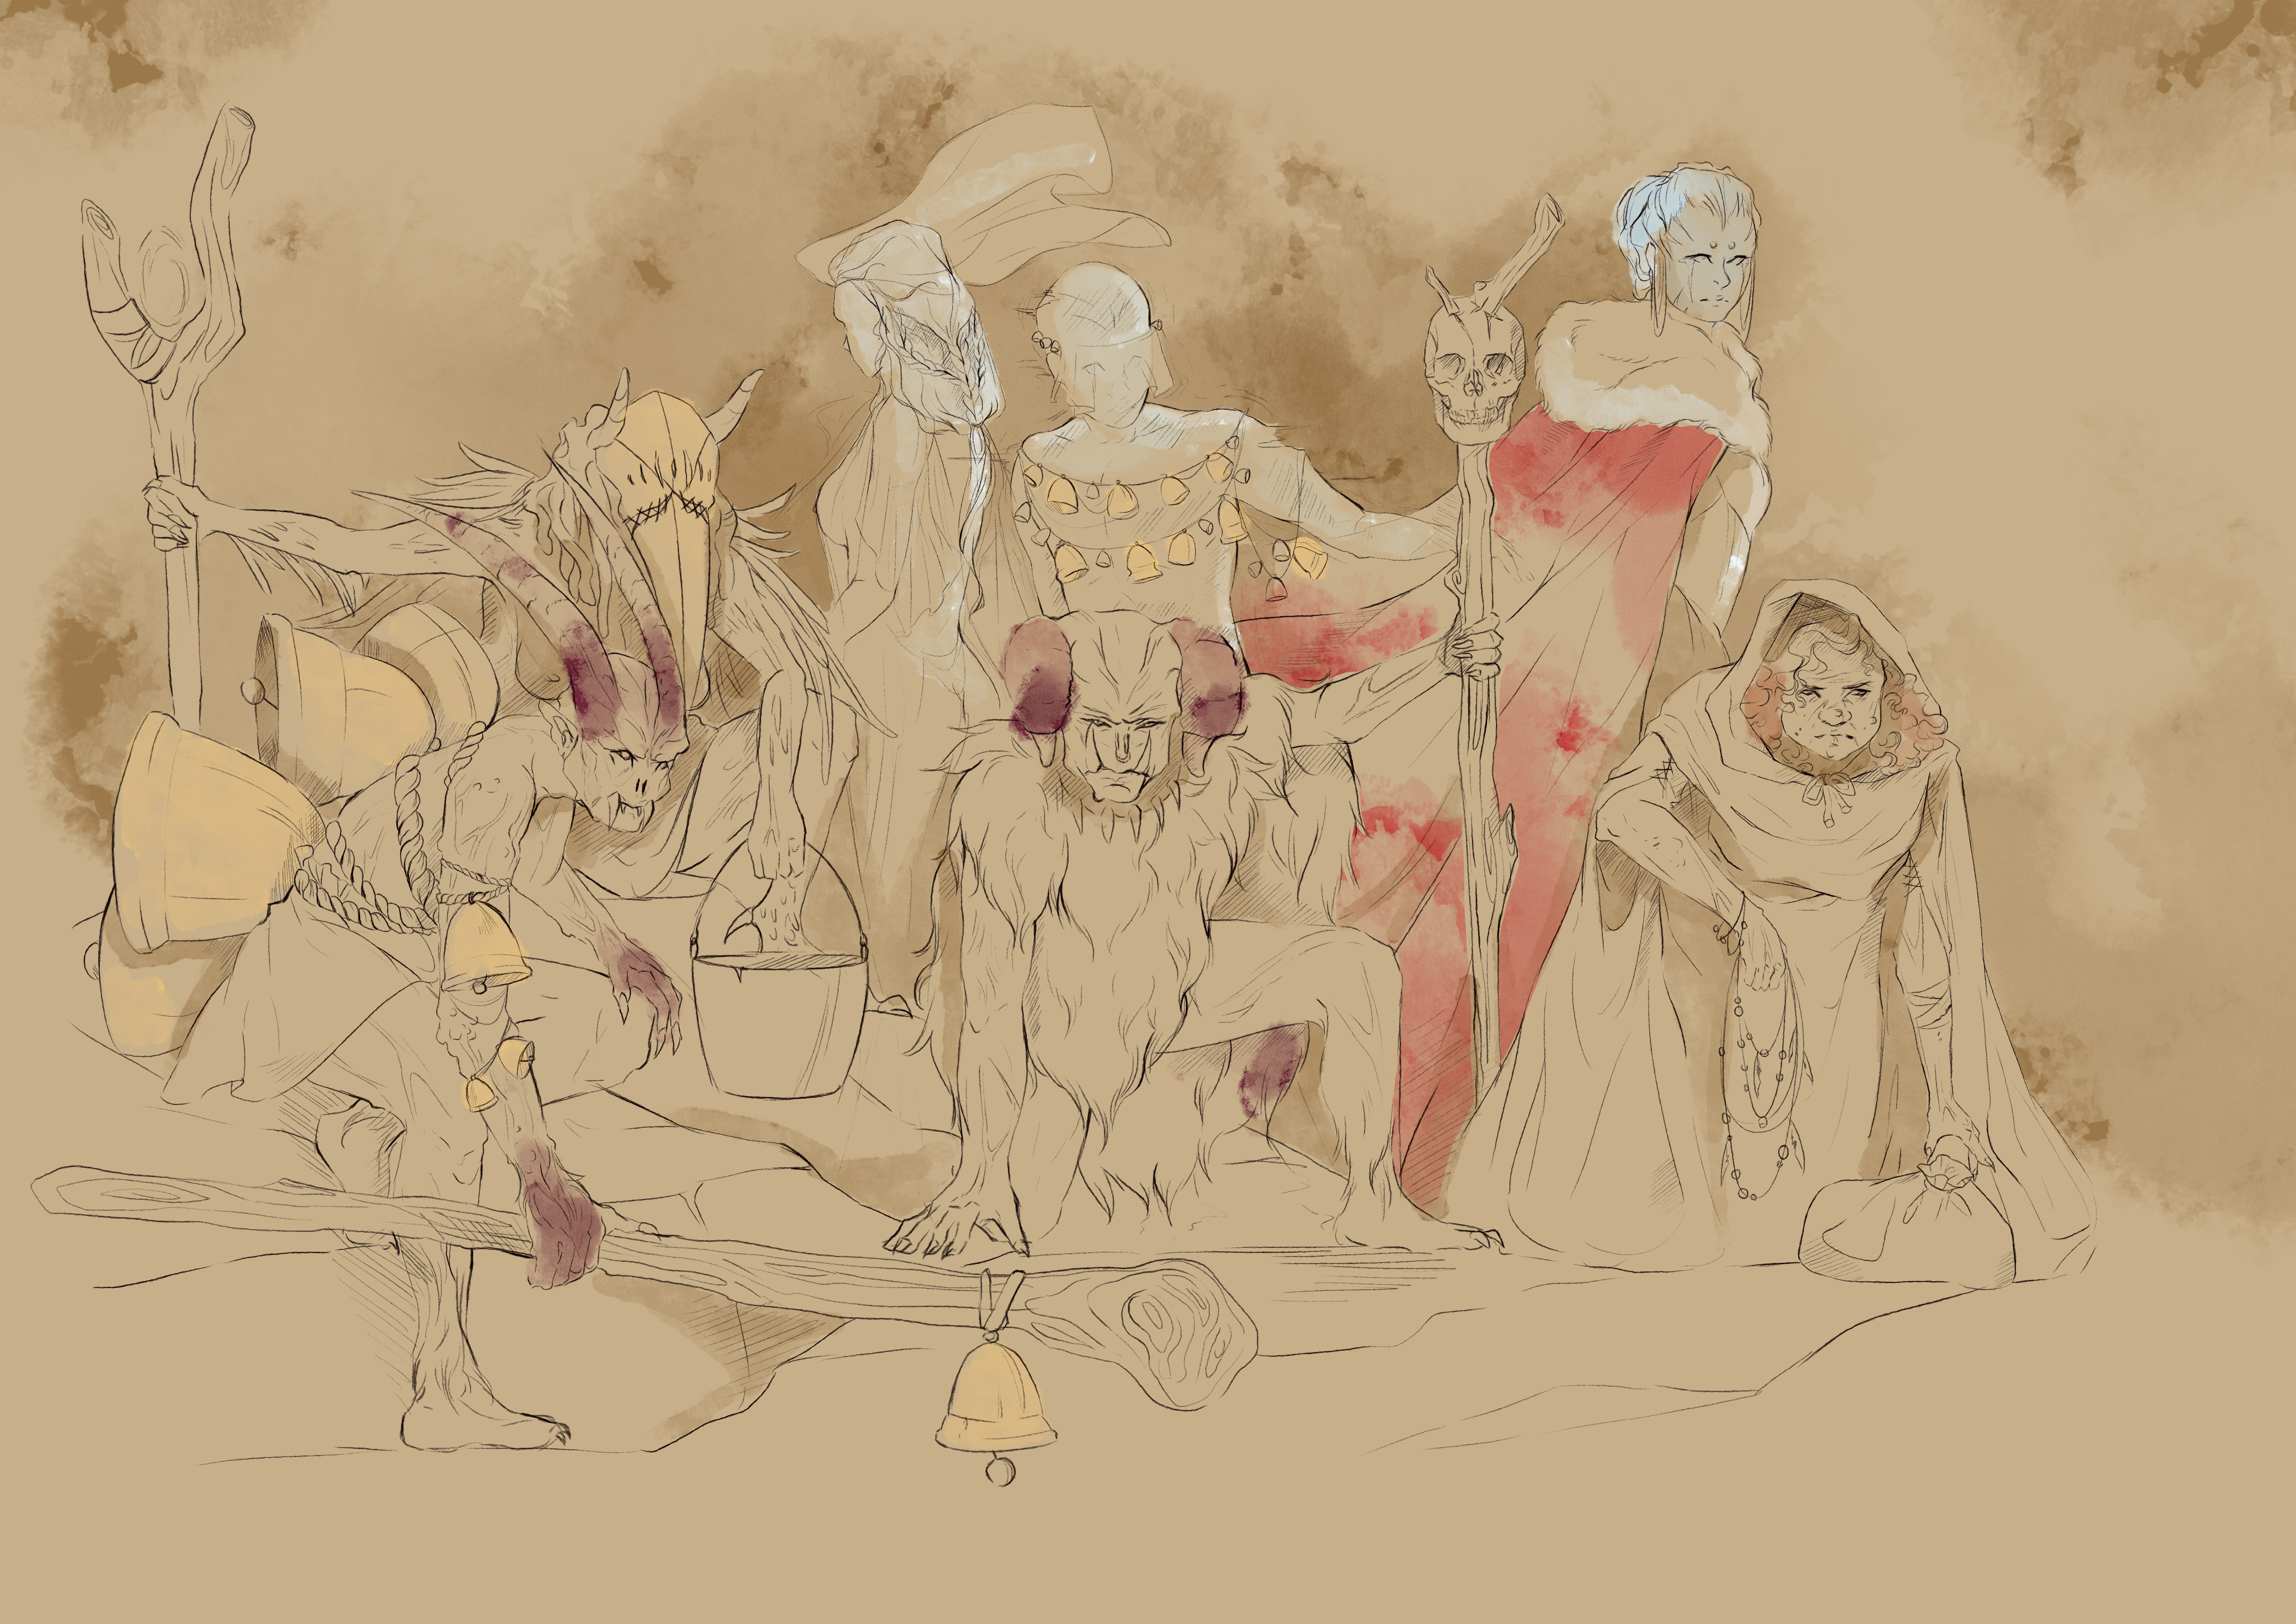
\includegraphics[width=\paperwidth,keepaspectratio]{media/perchten.png}
    }
    \par
    The Perchten of Aror: Habergoas, Schnabelperchten, White Maid, Bell
    Ringers, member of the Wild Hunt, Perchta, and a Bärbele.
\end{figure*}

\subsection{Percht}
\label{sec:Percht}

\emph{Percht} (plural ``perchten'') are ancient souls that inhabit the
\nameref{sec:Toralian Highlands}, and the \nameref{sec:Dirgewood}. They
are ancient souls that roam the forest and the mountains, that can manifest
humanoid bodies and figures when they wish to interact with other mortal
beings.

Generally perchten can be categorised into two groups: \emph{Schiachperchten},
which is Highland dialect for ``ugly perchten''. They often appear with
horribly distorted, ugly, animal-like appearance and are generally considered
evil and cruel. \emph{Schenperchten}, which means ``beautiful perchten'', on
the other hand are considered good, helpful and supportive. Schenperchten
always appear in normal humanoid form (for example as an old human crone
living by herself in a wood), and prefer to remain unnoticed. Both kinds of
perchten have incredibly powerful souls, and thus any \hyperref[sec:Soul
  Magic]{soul magic} that reveals souls, will also identify actual perchten in
disguise.

Perchten are not a race per se, but a collection of powerful individual souls
that roam the forests, caves, mountains, and valleys. While the evil ones might
cause mischief, harm and grief, the beautiful ones might actually help and aid
travellers and villages.

\subsubsection{Bell Ringers}
\label{sec:Bell Ringers}

The \emph{Bell Ringers} (or ``Gleckler'' in the Highlands) are a small group of
good Perchten (``Schenperchten'') who only appear when the evil Perchten
of the Wild Hunt begin to set out to hunt. They are free souls that shine
in a bright yellow light, and wander through towns and cities in the Highlands
warning the living inhabitants with a bell and rhyme to stay safe while
the wild hunt are afoot. The bell ringers are also known to reside in town
squares until the wild hunt is officially over, or even attempt to bring the
wild hunt to a premature end by chasing away the Schiarchperchten hunters. The
bell ringers only speak cryptic rhymes in old Teranim warning anyone about
the hunt, and disappear again as soon as the hunt is over. Many shamans of the
\nameref{sec:Old Ways} believe that bell ringers where once killed by the
hunters, and now wish to spare others of that fate. Worship, honouring and
giving sacrifices to the bell ringers is considered in an integral part of the
faith of \nameref{sec:Marwaid} and the \nameref{sec:Old Ways}.

\subsubsection{Bärbele}
\label{sec:Barbele}

The \emph{Bärbele} is a perchten with a distinct female appearance. It often
wears ragged, torn clothing, a colourful apron, and a beautifully carved
wooden mask. They are often ``armed'' with a broom and a woven basket, and
announce their arrival by ringing bells. They arrive at villages in small
groups near the end of the year and begin to clean the streets taking anything
with them that they consider litter. They then carry those items away and
build a shrine to \nameref{sec:Marwaid} near the village. While some might be
annoyed at the theft of their belongings, many see the arrival of these
perchten as a sign that worship Marwaid has been neglected in the last
year. They are generally harmless unless they are attacked first, or someone
attempts to steal from them.

\subsubsection{Frau Perchta}
\label{sec:Frau Perchta}

Mother Perchta (``Frau Perchta'' in dialect and old Teranim) is the supposed
mother and patron of all perchten gestalts that roam the region. She is
generally described as a good spirit that appears in the form of an old woman
or crone. Several tales about her exist in the stories of the \nameref{sec:Old
  Ways}, but most depict her as an older lady that punishes those that are
lazy and rude, while giving to those that work hard and are humble in spirit.
Throughout the stories and traditions of the \nameref{sec:Old Ways} she is
considered an aspect of \nameref{sec:Nyddwr}, as Frau Perchta rewards those
that work hard to earn their good future. She often visits towns, farmsteads,
villages and hammocks in disguise, or can be found living deep in the mountains
or woods as an old lone crone.

\subsubsection{Habergoas}
\label{sec:Habergoas}

\aren{Many know these by their mystical ``leader'' called \emph{Krampus}.}

The Habergoas, which combines the old Teranim words for ``he goat'' and ``she
goat'' into one name, is a horrific huge creature with a goat head, humanoid
torso and legs of a horse. It has either white or black fur, and always walks
on two legs while carrying a huge woven basket on its back. Its visage is
often a horribly disfigured face of a goat, and it is considered an evil
Schiachperchten. Habergoas is often armed with a long walking and fighting
stick on which hangs a bell that it ring loudly to announce its arrival. It
will wield that stick and its heavy bell much like one would a heavy flail. It
will wander into towns and villages, often at the beginning of winter, and
demand sacrifices from the villagers and towns folk or it will start abducting
people, especially children. It will not stop terrorising villages and people
until it finds the sacrifices to be sufficient.

The Habergoas is a respectable fighter, and its half-goat body has
considerable bodily strength and resilience. Fighting off a Habergoas might
just work, or it will just be angered even more doubling and tripling the
sacrifices required to appease it. The Habergoas will however recognise when
humanoids, especially younger ones who seek to prove their fighting spirit,
wish to brawl, and will use non lethal force in combat. To many young of the
Old Ways it is a great source of pride to have stood their ground against a
Habergoas, regardless of whether that attempt was successful or not. If the
Habergoas is impressed by the fighting spirit of the young, it might just
leave without taking any sacrifices.

\subsubsection{Schnabelperchten}
\label{sec:Schnabelperchten}

The Schnabelperchten (lit. beak or pecker perchten, but often simply called
``crow spirits'') are evil perchten (Schiachperchten) that arrive often in
groups at the beginning of a new year. They have humanoid bodies, often
covered in thick linen clothes. Their body shape suggests that there are male
and female crow spirits. Their heads are distinct by being absolutely
featureless, except for a huge (half a metre) white beak as a mouth. They do
not speak, but will herald their arrival with loud and rather distinct
crowing. Schnabelperchten further carry four items with them: A broom, a
dustpan, a large woven pannier that is carried on their backs, as well as an
oversized pair of scissors. They will knock on doors and windows, demanding
entrance. If entrance is not granted they will simply let themselves in, and
walk around the house inspecting its cleanliness. Should Schnabelperchten find
dust or dirt (apart from what they carried in themselves) they will clean it
up, gut the owner of the house with their scissors, and replace his entrails
with the dirt and stones before sewing up his stomach again.

Among all the Schiachperchten the crow spirits are the most feared and hated,
and have in recent years been actively hunted and killed by the knights and
priests following the \nameref{sec:Order} as well as the church of
\nameref{sec:Lor}. It is unknown why they act in this manner, especially since
their punishment is draconian compared to the offence of having a dirty house.

\subsubsection{White Maid}
\label{sec:White Maid}

The White Maid, is a mysterious good spirited Percht, that either randomly
wanders into town, or appears in large estates or castles. She is always a
young, beautiful woman with white hair, dressed in a spotless white dress. The
white maid loves children, and will often play with them, sing them songs,
teach them, or tell them the stories. She is a great teacher, and often
teaches the children morals, and the history and stories of the
\nameref{sec:Old Ways}. Within the religion of the Old Ways, she is seen as an
avatar of \nameref{sec:Forun}.

\subsubsection{Wild Hunt}
\label{sec:Wild Hunt}

The \emph{Wild Hunt} (``Wüdjogt'' in Highlands) are a collection of Perchten,
and nature spirits, that roam the forests of the Highlands to hunt. They
primarily hunt undead, but will hunt anything unfortunate enough to cross
their paths, even humanoid creatures. They are thus considered evil
Schiachperchten. They hunt mostly with bow and arrow, and sound their very loud
and distinct hunting horns, and drums when setting out for hunts. The wild hunt
will continue until the Perchten are satisfied with their prey, or until they
are driven away by the bell ringers. The hunters cannot be reasoned with, but
may be defeated upon which they retreat back into the soul well.
